%!TEX root = ../master.tex

\chapter{Implementation}\label{ch:implementation}
Our development chapter. \todo{Better introduction needed here.}

\section{Rear Diffused Illumination} \label{sec:RDI}
\begin{figure}[!h]
\centering	\includegraphics[width=0.5\textwidth]{sketchAugmentedBoard}
 \caption{An sketch of our RDI table.\label{Fig:sketch}}
\end{figure}
The interaction on the game board table will be based on rear diffused illumination as described in Multi-Touch Technologies \citep{multiTT}. This means, as shown in Figure \ref{Fig:sketch}, that infrared (IR) lamps will be placed underneath the table's surface, projecting IR light upwards. A webcam below the table will be equipped with a visible light filter obtained from a floppy disc, meaning it will primarily detect IR light. Furthermore, the table's surface, made of transparent material, needs a diffuser material just above or beneath it in order to diffuse the light. The purpose of this diffuser is to scatter the IR light and make objects hovering over the surface less visible to the camera. When an object touches the surface, the area of contact reflects more IR light than the untouched areas of the diffuser. This reflected light is captured by the camera, and can then be extracted as a BLOB. The diffuser has the additional purpose of facilitating a projection of the user interface from below.

\begin{figure}[!h]
\centering	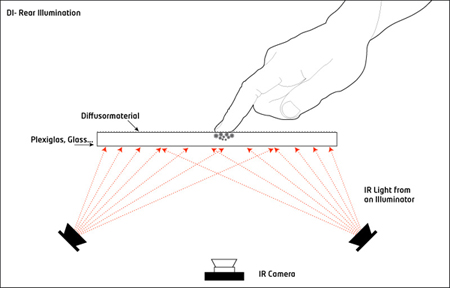
\includegraphics[width=0.5\textwidth]{RDItouch}
 \caption{Rear Diffused Illumination, illustrated NUI Group \citep{multiTT}\label{Fig:RDI}}
\end{figure}

Choosing such a solution has its advantages and disadvantages. First of all, there is no need for a silicone rubber overlay, called a compliant surface, which normally would be needed for a FTIR solution \citep{multiTT}, as described in the next section. There is also no need for soldering an LED frame, since we are using a diffuser in order to reflect the IR-light coming from below. The illuminators for that can be bought ready to go, so there is no need to build them. A disadvantage comes from the RDI having difficulties with getting even illumination, since the IR-lights might not cover the table's surface completely, or they might overlap, causing areas with an excessive amount of reflected IR light. This can result in false BLOBs, as well as BLOBs of lower contrast which are hard to detect. All this can challenge the software's detection of the desired BLOBs.

\subsection{Multi-Touch technologies alternatives}\label{technologiesAlternatives}
Besides RDI, other solutions are presented in Multi-Touch Technologies \citep{multiTT}:

\textbf{Frustrated Total Internal Reflection:} Instead of shining light from below, IR LEDs are projecting IR light directly into the acrylic glass from the side, which causes a total internal reflection. That means that until the user touches the surface, the IR light is totally reflected inside the glass. Once the surface is touched, the light rays are 'frustrated', causing the light to go downwards, which a webcam can capture in the same manner as with RDI. FTIR requires soldered IR LED, acrylic glass, a baffle to hide leaking LED light from sides of the glass, a diffuser, and a compliant layer which acts as a touch proxy, since it will improve the performance of FTIR.

This solution does not require an enclosed box, has strong contrasted BLOBs, allows varied BLOBs depending on touch pressure, and can with a compliant surface be used with even smaller tips than fingers have. Furthermore, is does not have the problem of uneven illumination which is present with RDI. However, it requires a soldered LED frame and a compliant surface, which makes it an unpractical solution.

\textbf{Front Diffused Illumination:} Visible light is shined from above the touch surface. This requires a glass surface with a diffuser layer. The camera captures the shadow created by touches of the surface. This solution requires no compliant surface, no LED frame, no soldering and no enclosed box, which makes it the simplest set-up of them all. It can make use of any transparent material and it can track fingers both touching and hovering, since both still creates the shadow needed.

The problems with this solution is that  it cannot track objects. It also has difficulty avoiding false BLOBs and get even illumination, which makes it less reliable. This solution is not optimal when working on a digital board game, as the camera would catch too many shadows without players touching the board. This would cause problems, as players need to be able to gesticulate to each other during the game.

\textbf{Laser Light Plane:} This solution works by having a 1mm thick plane of IR light shined right above the surface by lasers. Whatever is in close contact with the surface, for example a fingertip, causes the light to scatter downwards to be seen as a BLOB by a webcam. Just as with front DI, LLP has a simple set-up which can use any transparent material as surface, and does not require a LED frame, an enclosed box or a compliant surface. It is also described as a cheap solution. The problems with LLP lies it its inability to track objects and being pressure sensitive. More importantly, it can have problems with several touches or objects can block the lasers for each other. This could be a problem, if we for example had game pieces on the board, which makes this solution unusable for this project's problem. 

\textbf{Diffused Surface Illumination:} Almost as with the FTIR set-up, but without a compliant surface, the DSI make use of a Endlighten acrylic. This kind of acrylic redirects light evenly out to the surface of the surface.  Touches on the surface disrupts the even light where they happen, which creates contrasts that can be captured as BLOBs by a webcam. DSI is also pressure sensitive, due to the nature of how touch influences the light, and it can detect objects. Its disadvantages lies in the Endlighten acrylic's price, possible size restriction because of the special acrylic's softness and a lower contrast than the FTIR and LLP. Especially the restrictions and lower contrast made this solution less favourable than the others.

\textbf{LED Light Plane:} With some similarities to FTIR and LLP, LED-LP has IR LED from the sides, but without an acrylic layer to move through, it is instead shined over the touch surface, which can be of any transparent material.

\section{Physical Design} 
\begin{figure} [!h]
\centering 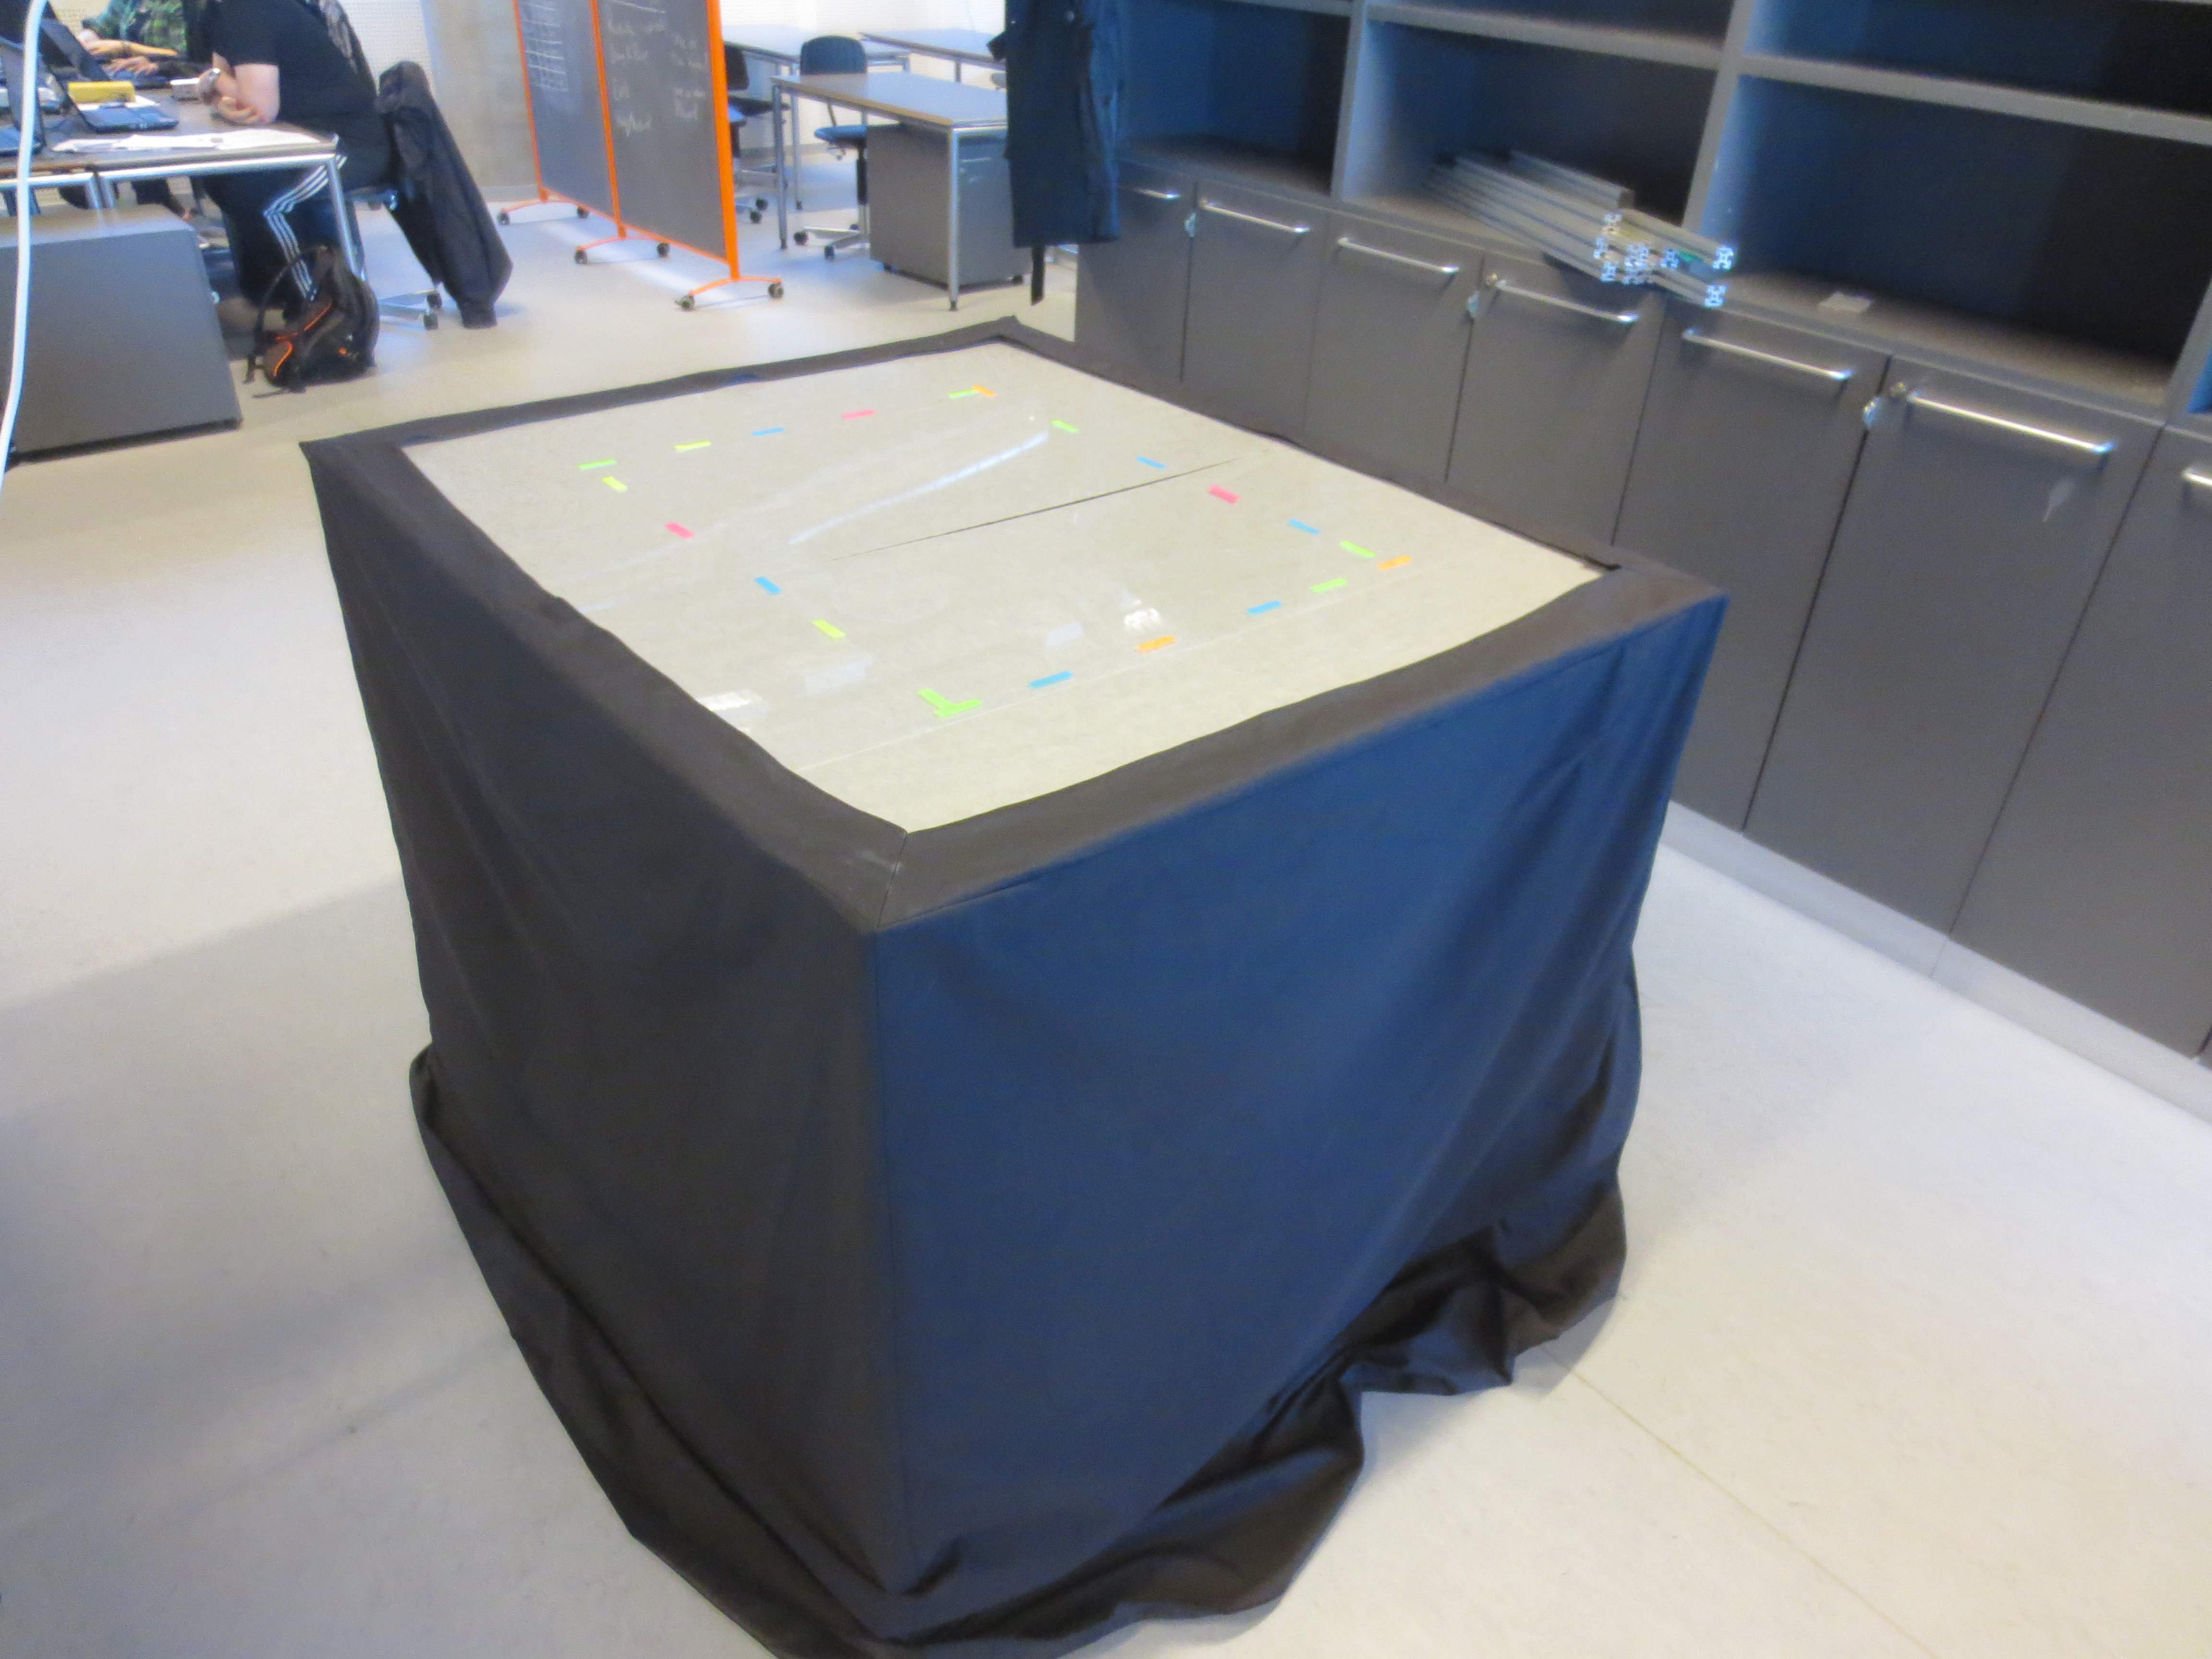
\includegraphics[width=0.5\textwidth]{Table}
 \caption{The touch table \label{Fig:Table}}
\end{figure}
This section will describe the physical aspect of our product.
The table's surface is made from acrylic glass, and below are four IR lamps, as well as a webcam with a visible light filter, and a short-throw projector, which will project images on the table. The webcam and IR lamps are there to facilitate RDI, as explained in Section~\ref{sec:RDI}. All these elements are placed in a manner that spreads the IR light from the lamps as evenly as possible.

The outer frame of the table is constructed from 3 different lengths of aluminium extrusions, giving the table a final size of 120 x 102 x 89 cm.
In order to keep outside IR light from disturbing the image as much as possible, black cloth covers the table at the sides. The cloth has the additional benefit of making the projection from the short-throw projector clearer. 

As diffuser material, baking paper was chosen, as it is easily available. The paper is placed underneath the glass surface, as tight as possible, as placing it on top results in too much light being reflected by the acrylic glass into the webcam. If the diffuser is not attached tight enough to the glass, touching the surface does not result in enough IR light being reflected. The diffuser also works as a screen by blocking the light from the projector. 

\section{Image Processing}
To facilitate user interaction, a software module is needed to analyse a video input and recognize specific features and changes over time. As described in Section~\ref{sec:ReqSpec}, there are two main criteria for this software's minimum implementation. It needs to:
\begin{itemize}
\item Recognise which gesture is done when selecting player.
\item Recognise when a tile is selected for terraforming.
\end{itemize}

To do these, BLOBs need to be extracted from the video input through segmentation. Since it is difficult to create a uniform surface of reflected IR-light, it might be necessary to apply background subtraction to the input before segmentation. 

Furthermore, since this is a video feed rather than a static image, several of the methods in use will have to be looped. This leads to a three-step solution for processing the video input:

\begin{enumerate}
\item Prepare video frame for segmentation (Pre-segmentation).
\item Segment image (Segmentation, includes de-noising/smoothing).
\item Conditionally change data depending on the BLOB analysis
\end{enumerate}

\subsection{Pre-segmentation}
To prepare the video feed for segmentation it is necessary to do image subtraction. For this project background subtraction is most useful since the point is to detect static BLOBs and not movement and for that an empty background is needed. 

\begin{figure}
	\centering
	\begin{subfigure}[b]{0.3\textwidth}
	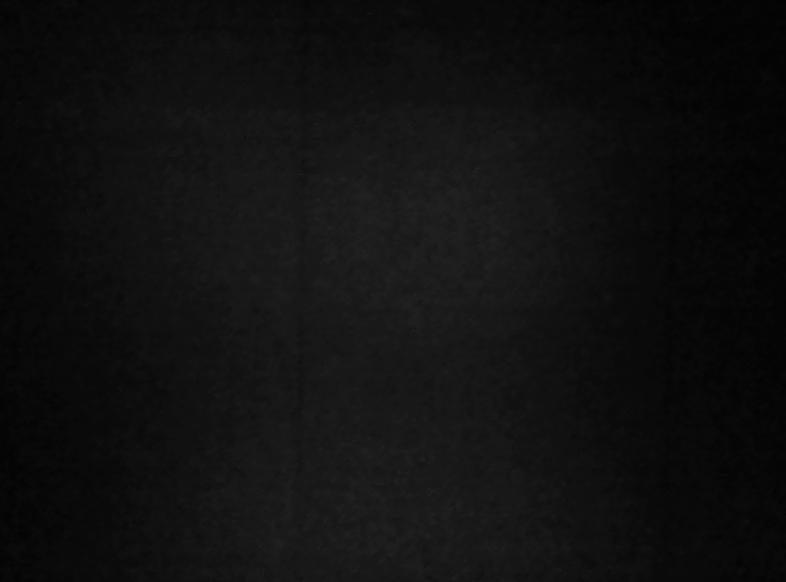
\includegraphics[width=\textwidth]{UnSub}
		\caption{\label{Fig:UnSub}}
	\end{subfigure}
	\begin{subfigure}[b]{0.3\textwidth}
	
\includegraphics[width=\textwidth]{BackgroundSub}
		\caption{\label{Fig:BackgroundSub}}
	\end{subfigure}
	\caption{Picture \textbf{(a)} is the input image and picture \textbf{(b)} is the background subtracted image\label{Fig:Subtract}}
\end{figure}

Background subtraction works by using the first image in the video as the referencing image r(x,y) and then subtracting that from the current image f(x,y), using this formula: \textit{g(x,y) = f(x,y) - r(x,y)} \citep{moeslund_introduction_2012}. 

\subsection{Segmentation}
There are several methods for segmenting images. The relevant methods are discussed in this section. 

As the project deals with video as opposed to static images, there is an issue with image noise. As the input from the camera is constantly updating, the noise is not static, and is not completely removed by teh initial background subtraction. Therefore, a smoothing filter is necessary, so more noise can be negated. In this case, a Gaussian blur was implemented.

\begin{figure}[h!]
\centering 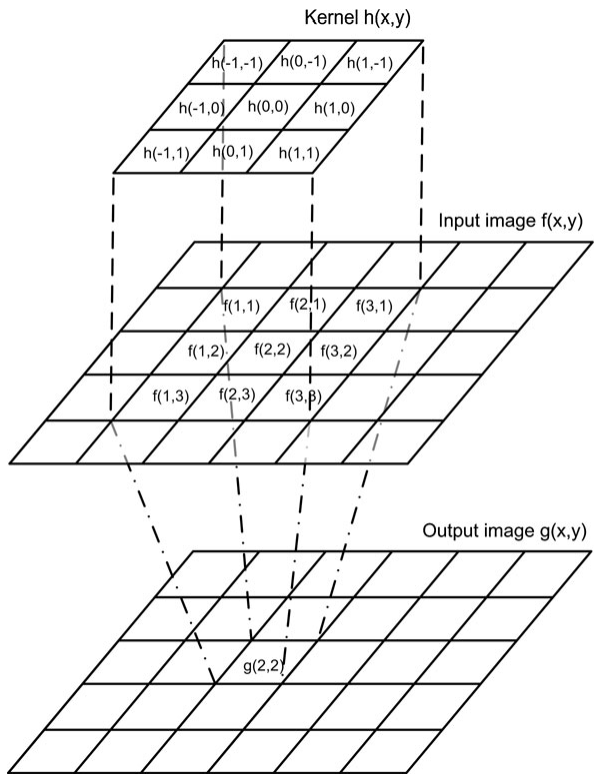
\includegraphics[width=0.3\textwidth]{Correlation}
\caption{A visualisation of correlation \label{Fig:Correlation}\citep{moeslund_introduction_2012}}
\end{figure}

A Gaussian blur is a correlation-based image processing operation, making use of a kernel. This works, by having the kernel overlay on top of the pixels of the image that is processed. That way, the kernel cells are each paired with a pixel, which through calculations gives a new pixel value. This process is illustrated in Figure \ref{Fig:Correlation}. The Gaussian kernel, displayed in Figure \ref{Fig:Gaussian}, is a kernel with a specific pattern. This pattern gives more weight to the pixels paired with the centring kernel values, thereby giving them more influence in the image processing. It is used to remove detail from an image, which as mentioned earlier is useful to remove noise.

\begin{figure}[h!]
\centering 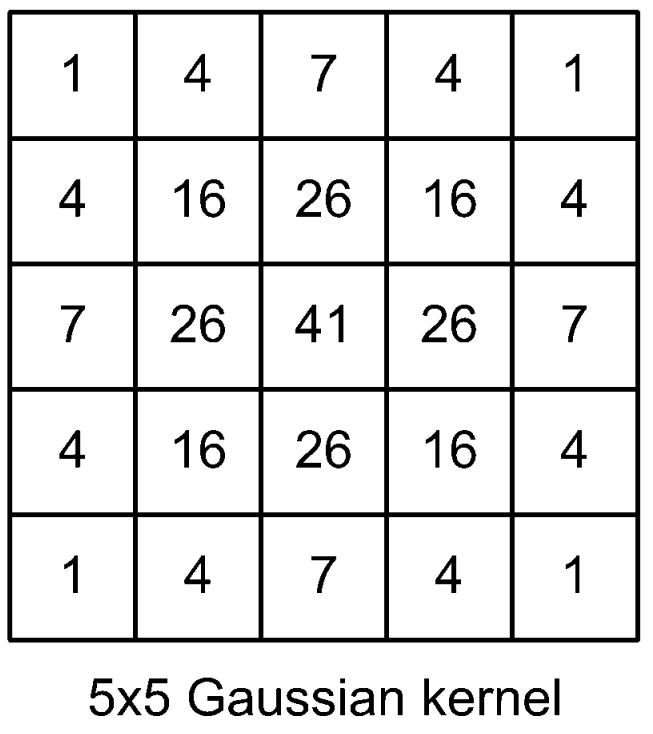
\includegraphics[width=0.3\textwidth]{Gaussian}
\caption{A 5x5 Gaussian kernel pattern \label{Fig:Gaussian}\citep{moeslund_introduction_2012}}
\end{figure}

After smoothing and removal of noise, the video feed needs to be thresholded, so what the computer needs to detect becomes white, and all that is irrelevant is black. As described in Section~\ref{sec:RDI}, the hardware setup uses RDI with IR light sources, and a visible light filter on a web camera. What is thresholded is therefore the section of the image, which contain the hand that is placed on top of the board.
 
In an ideal thresholded image, the histogram will have two distinct 'mountains' of pixel values, that is to say, there will be two groups of pixels that, within each group, have a similar brightness while at the same time the groups themselves are isolated from each other. In the case of this project, the image produced is expected to have bright spots where the board is touched, on a dark plane which is to be considered the background.
 
 
\subsection{BLOB analysis}
To remove the last noise and make the BLOBs more visible, a morphology method is deployed. The chosen method \textit{opening}, consists of two operations: an \textit{erosion} operation and a \textit{dilation} operation \citep{moeslund_introduction_2012}. By first calling the erosion operation, most of the remaining noise BLOBs are removed, but the BLOBs necessary for the detection are also reduced. This is when the dilation operation is called, which then dilate the already eroded BLOBs which affects the BLOBs necessary for the detection but should not affect the noise BLOBs since they are either too small or entirely gone for the dilation operation to catch them. 

Afterwards the remaning BLOBs seen by the computer needs to be identified as the BLOB needed for the project, in contrast to what noise there might be left. This is done, by giving each seen BLOB a convex hull. A convex hull of a BLOB is, as described by Moeslund, "\textit{is the minimum convex polygon which contains the BLOB. It corresponds to placing a rubber band around the BLOB.}" Calculations can then be made on this polygon. In this project, the area of the convex hulls are calculated. By then filtering the convex hulls by size, ignoring those that have a small area, a BLOB from a hand can be detected.

\section{Rendering of game board}
\begin{figure}[h!]
\centering 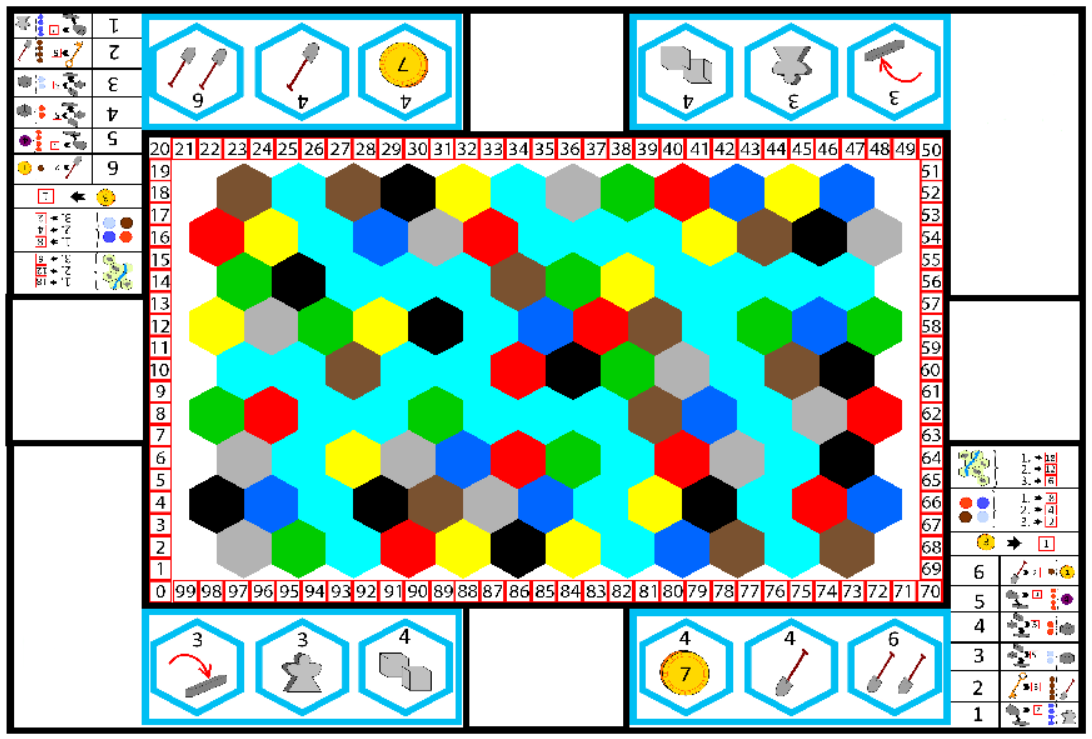
\includegraphics[width=0.5\textwidth]{BoardWithTilesNoUndo}
\caption{The game board \label{Fig:Board}}
\end{figure}
In order for the program to be able to change the game tiles through terraforming, it must have access to them from the start. This is done, by having the program render out all the tiles. The border around the actual tiles are made from a background image, which is imported as is. This image contains the outline of a player area for each player, the point counter, and the border for each exclusive action. 
\begin{figure}[h!]
\centering 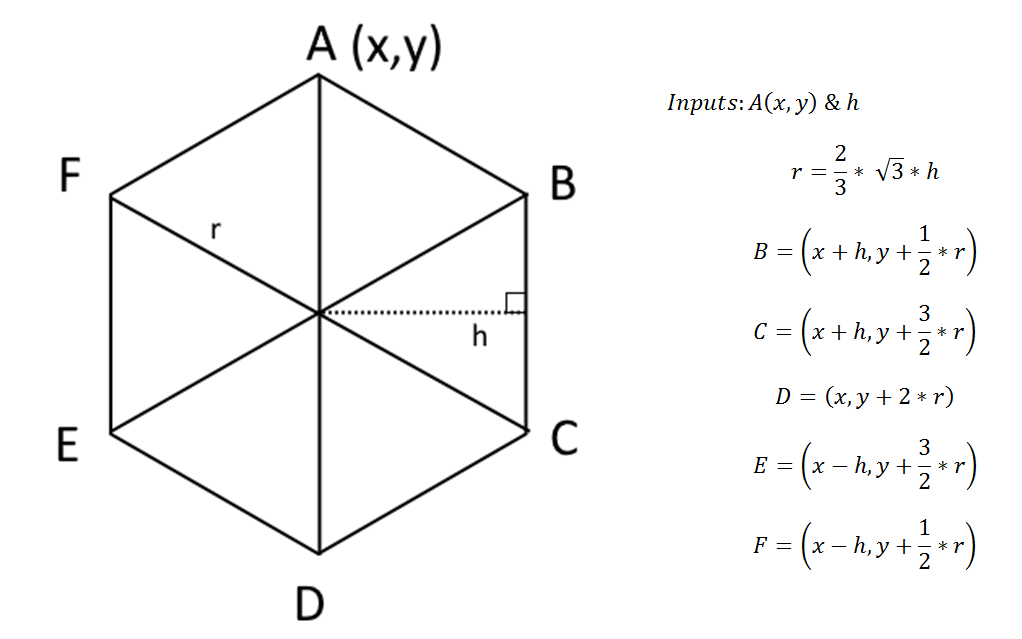
\includegraphics[width=0.7\textwidth]{HexWithMath}
\caption{Relations between height and points in hexagon \label{Fig:HexWithMath}}
\end{figure}

On top of this image is the rendering of the tiles themselves. This is done with a function, which takes a two-dimensional coordinate, the height of the hexagon, the image on which to draw on, and a colour as parameters. The function calculates the radius based on the height input, which is then used to calculate the relations between the coordinate input and the remaining coordinates. Then the function fills it with the given colour. The equations used to calculate the points in the hexagon are shown in Figure \ref{Fig:HexWithMath}.

With this method, the program renders out the board row by row, saving the coordinate of the A-point of each tile and the colour in two different arrays. The resulting rendered board is what is shown in Figure \ref{Fig:Board}.